%% Adaptado de 
%% http://www.ctan.org/tex-archive/macros/latex/contrib/IEEEtran/
%% Traduzido para o congresso de IC da USP
%%*****************************************************************************
% N�o modificar

\documentclass[twoside,conference,a4paper]{IEEEtran}

%******************************************************************************
% N�o modificar
\usepackage{IEEEtsup} % Definies complementares e modificaes.
\usepackage[utf8]{inputenc} % Disponibiliza acentos.
\usepackage[english,brazil]{babel}
%% Disponibiliza Ingl�s e Portugu�s do Brasil.
\usepackage{latexsym,amsfonts,amssymb} % Disponibiliza fontes adicionais.
\usepackage{theorem} 
\usepackage[cmex10]{amsmath} % Pacote matematico bsico 
\usepackage{url} 
%\usepackage[portuges,brazil,english]{babel}
\usepackage{graphicx}
\usepackage{amsmath}
\usepackage{algorithm}
\usepackage{algpseudocode}
\usepackage{mathrsfs}
\usepackage{amssymb}
\usepackage{color}
\usepackage[pagebackref=true,breaklinks=true,letterpaper=true,colorlinks,bookmarks=false]{hyperref}
\usepackage[tight,footnotesize]{subfigure} 
\usepackage[noadjust]{cite} % Disponibiliza melhorias em citaes.
%%*****************************************************************************
\usepackage{epstopdf}%====================================
\usepackage{cite}%====================================
\usepackage{hyperref}%====================================
\usepackage{pgfgantt}%====================================
%\usepackage{subfigure}%====================================
\usepackage{graphicx}%====================================
%\usepackage{caption}%====================================
%\usepackage{subcaption}%====================================
\usepackage{subfigure}
\usepackage[hypcap]{caption}
\usepackage{float} 
\usepackage{gensymb}

\begin{document}
\selectlanguage{english}
\renewcommand{\IEEEkeywordsname}{Keywords}

%%*****************************************************************************


\urlstyle{tt}
% Indicar o nome do autor e o curso/n�vel (grad-mestrado-doutorado-especial)
\title{Project 1 - Odometry and Feature Extraction}
\author{%
 \IEEEauthorblockN{Gabriel Capiteli Bertocco\IEEEauthorrefmark{1},Thales Mateus Rodrigues Oliveira\IEEEauthorrefmark{2},Elisangela Silva dos Santos	\IEEEauthorrefmark{3}}
 \IEEEauthorblockA{\IEEEauthorrefmark{1}%
                   Computer Science - PhD Program -
                   E-mail: gabriel.bertocco@ic.unicamp.br \\, \IEEEauthorrefmark{2}%
                   Computer Science - Masters Program -
                   E-mail:ra148051@students@ic.unicamp.br \\, 
                   \IEEEauthorrefmark{3}%
                   Computer Science - Special Student -
                   E-mail:ra149781@ic.unicamp.br}
}

%%*****************************************************************************

\maketitle

%%*****************************************************************************
% Resumo do trabalho
\begin{abstract}
    In this project, the group was given task of building an odometry and feature extraction system for an autonomous wheeled robot, P3-DX. The mentioned goals are the basis for robot performance in the environment, as they guarantee robust and reactive operation in real time. Reliable enough odometry leads to trustworthy features, hence more complex actions such as control, mapping and navigation. To fulfill the requirements, the algorithm implemented deals with the kinematic model of the robot for odometry calculation, its sensors for acquiring information from the environment and a RANSAC algorithm to extract features. The V-REP simulator was used to test the developed structure. The group was able to generate different odometry qualities depending on sensor usage, with good results in the best case. The point extraction performs well, considering that the current position of the robot is reliable. The feature extraction algorithm is able to calculate obstacles such as walls and supports of objects, not considering possible outliers.
\end{abstract}

% Indique três palavras-chave que descrevem o trabalho
\begin{IEEEkeywords}
    autonomous systems, robot kinematics, robot sensing systems
\end{IEEEkeywords}

%%*****************************************************************************
% Modifique as seções de acordo com o seu projeto

\section{Introduction}
\subsection{Background and motivation}

The study of mobile robotics is of great importance and current, since there is growing demand and investments related to the area in various sectors of technology\cite{siegwart2011introduction}.
Studies, research and development made a major leap in technologies involving the application of mobile robots. Today, there are domestic, industrial, urban, militar and security applications, exemplifying the great importance of mobile robots today.
\par
The area of Autonomous Robotics, that is, the performance of robot actions through space without any external assistance from humans, has gained importance as they can be extremely advantageous in many applications, reducing many expenses and increasing reliability.
\par
In order to implement a robust autonomous system, the robot has to be able to execute a simple pipeline execution, which consists of sense, plan and act. The system needs to have the capacity of acquiring information from the environment (which is done by readings of sensors, such as cameras, Ultrasonic sensors, LIDARs) and itself (like encoders, gyroscopes\cite{Gyroscope}, temperature and so on), decide what to do based on these readings, and perform the decided action.
\par
The ability of a mobile robot to move in an environment is one of robotics' most basic and important activities. Successful locomotion is linked to the use of reliable sensors to provide the correct robot position information. With the right position information, the robot can make safe decisions, such as moving to interest points, map an unkown environment, perform specific actions it was supposed to (\textit{e.g.:} deliver of machinery for industrial robots, identifying victims and their spots in desaster zones, map structures in cities).
\par
To be able to move with accuracy to its goals, the robot relies on a good odometry\cite{estherclasses} calculation, which consists in being able to analyze, by direct kinematics, its position and orientation based on the volocity applied in its wheels, in the case of wheeled robots. 
\par
Sensing the environment is also an important issue for autonomous robots. Choosing the right sensor is of paramount importance for the application, in order to avoid obstacles, do reliable mapping, and so on. With the information extracted from those sensors, local features from the environment can be processed, such as walls, unleveled structures, objects of interest, and others. 


\subsection{Work Objectives}

The general objective of this work is to build an odometry and feature extraction systems able to estimate the position of the robot over time, and also to process information obtained from the sensors, for the robot Pioneer P3-DX, shown in figure \ref{fig:p3-dx} to be tested in the V-REP \cite{robotics2016v} Robotics Simulator.

\begin{figure}[ht]
    \centering
    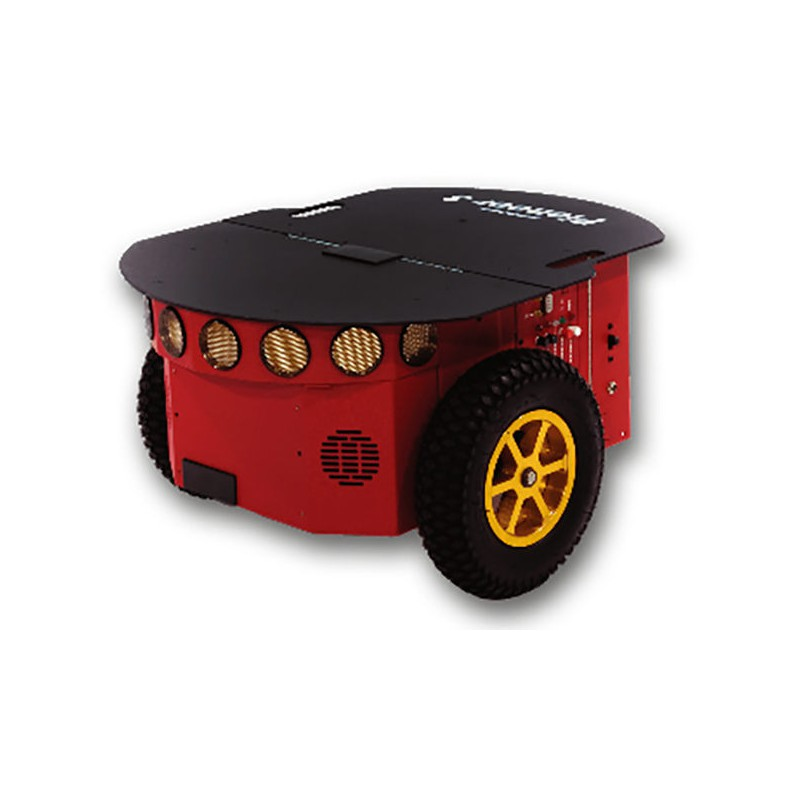
\includegraphics[width=0.3\textwidth]{figures/robot-mobile-pioneer-3-dx.jpg}
    \caption{Pioneer P3-DX.}
    \label{fig:p3-dx}
\end{figure}

\subsection{Organization}
The following work is divided into 4 sections. Section II deals with points extraction from the scene, section III with the Odometry, section IV talks about the evaluation of Points Extraction and Odometry together, and section V discuss the Feature Extraction algorithm. Those sections explain the implemented algorithms, related tests and discussions. Section VI sums up the work with the conclusion. 
\section{Points Extraction}

The robot that we are working here has two kind of distance sensors: laser sensor and ultrasound sensor. To perform
the point extraction we used only the laser sensor since its distance range from the robot is greater than the one 
returned by the ultrassound sensor. Besides, laser sensor get 1500 points at once in each calling to the reading data 
function as long as we have only 16 points got by the ultrassound sensors. \par 
The laser sensor has its own reference system which is not the same of the global reference system when the robot is 
in different positions. So, to localize the points extracted from the enviroment we must have a standard
coordinate system in which we will project all the points in a same space in order to have a consistent representation
of the enviorment independent of the robot orientation. In this case, our standard system is the global reference system
of the scene, therefore, given the coordinates of a point detected by the sensor we need to project this point from the
local coordinate system of the sensor to the global reference system of the scene. Basically, we need to apply two 
transformation in the point: rotation and translation. \par
Once a point is detected by the laser sensor, we can access its coordinates on the local coordinates system. To get its 
values in the global one we need, firstly, to rotate the local system in order to have the same directions. 
We performed this applying the following equation to a point $ P_{0} = (x_{0}, y_{0}) $ detected by the 
laser sensor:

\begin{gather}
 \begin{bmatrix} x_{1} \\ y_{1} \end{bmatrix}
 =
  \begin{bmatrix}
   \cos \theta & -\sin \theta \\
   \sin \theta & \cos \theta 
   \end{bmatrix}
   \begin{bmatrix} x_{0} \\ y_{0} \end{bmatrix}
\end{gather}

Where $ \theta $ is the rotation angle between the local e global reference frame and $ P_{1} = (x_{1}, y_{1}) $ is the 
same point detected by the laser but referenced in the rotated local system. It is importante to realize that the $ z $ 
coordinate is always the same value for all points in the same reference system since the robot does not change its 
altitude (robot does not climb up or go down), that is why we did not need to put it on the account. Besides, coordinate 
systems of the laser sensor has exactly the same directions of the coordinate system of the robot, that is, it is 
exaclty over the center of the robot. So we are always assuming that the system origin of both are the same. To get the 
coordinates of the point in the global coordinate system we need only to translate the local reference frame for 
coincide with the global reference frame, which can be mathematically expressed in the following equation:

\begin{gather}
 \begin{bmatrix} x_{2} \\ y_{2} \end{bmatrix}
 =
   \begin{bmatrix} x_{laser} \\ y_{laser} \end{bmatrix}  
   +
   \begin{bmatrix} x_{1} \\ y_{1} \end{bmatrix}
\end{gather}

Where $ P_{laser} = (x_{laser}, y_{laser}) $ is the position of the laser related to global reference frame and $ P_{2} = (x_{2}, y_{2}) $ is the position of the point detected by the laser in the global frame. Now, the robot can move in any 
direction and all the points will be represented in the same system. So we proposed a trajectory to be followed by the 
robot in order to get into all parts (rooms) of the scene and get points from the whole enviorment. Once the robot 
finishes the trajectory we can see all the points representing the whole scene. This is shown in Figure \ref{fig:Points_Extraction}. 

\begin{figure}[h]
\begin{center}
    % \centering     %%% not \center
\subfigure[Upper view of the whole scene.]{\label{fig:real_scene}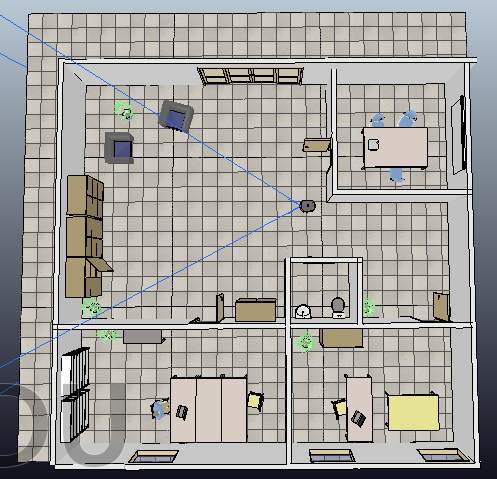
\includegraphics[width=0.22\textwidth]{figuras/W01Scene.png}} \hspace{0.1cm}
\subfigure[Points extracted from the scene.]{\label{fig:points_scene}\includegraphics[width=0.22\textwidth]{figuras/points.png}} \\
\caption{Result of Point Extracted compared to the real scene.}
\label{fig:Points_Extraction}
\end{center}
\end{figure}


\subsection{Discussion}
Since in each iteration we are getting 1500 points, we filtered them out in order to have only $ 10 $ points equally 
having the same angle between two consecutives ones. We tested with another values of downsampling and we concluded that 
even with 10 points in each iteration, we are having a good representation of the points of the enviorment. The 
downsampling has been done because sometimes many beams scan over the same part of the enviorment or even the same beam
might capture again the same point. This happens because of the high discretization of the laser sensor ($ 1500 $ points
at once), since we read the sensor in each iteration of the algoirthm, we could end up with 10 millions of points in a
short distance that robot goes by. This leads to lot of redundancy, memory consuming and time consuming in the feature
extraction stage. Therefore we chose to apply this downsampling strategy and we ende up with a lot of points but over the whole
enviorment. Figure \ref{fig:real_scene} shows us an upper view of the whole enviorment as long as Figure 
\ref{fig:points_scene} show us the points extracted from it. We see that the majority has been captured which allow us
to have a good representation and enough data for the feature extraction. Points that have not been scanned are mainly
the ones in rooms where the door is closed, for instance the bathroom, others are behind the wardrobes and in the upper
left nand right corners of the scene where the laser did not reach. Once we have the points extracted, we can perform the feature extraction.    

\section{Odometry}

Odometry is the tracking of the robot trajectory performed based on its sensors information. In this work, we used two
sensors to calculate the robot odometry: the encoders in the wheels and the gyroscope over the robot positioned exactly
over the robot's center in order to have the axes of the gyroscope and of the robot in the same directions. So, the
coordinates reported by the gyroscope frame will be the same reported in the robot frame. In fact, it could have a 
little difference in the altitude reported ($ z $ axe), however, since the robot does not change his altitude in the
kinematic model, we only worry with the $ x $ and $ y $ coordinates that are the same in both frames. So, three experiments have been performed 
to calculate odometry: based only on the encoders wheels, based only on the gyroscope and based on the fusion of both. 
In order to refine the results, we performed a filtering in the angles calculated by the sensors in the sense that we multiplied the angles 
by a factor in order to increase or decrease the angle value. This
has been done since we might have noise, errors, delays and some asynchronous behaviour between the python code and the V-REP simulator which could lead
us to bad acquired data. \par
When we are tracking the robot trajectory in the global frame, we need to describe the robot position based on three
values: $ x $ coordinate, $ y $ coordinate and the $ \theta $ angle between the $ x $ (or $ y $) axe of the robot (local 
frame) and the $ x $ (or $ y $) axe of the global frame. We are going to reference them as $ (x_{robot}, y_{robot}) $ 
and $ (x_{global}, y_{global}) $ respectively. When the robot goes from the position $ P_{}^{(k)} = (x_{robot}^{(k)}, y_{
robot}^{(k)}, \theta_{robot}^{(k)}) $ to position $ P_{}^{(k+1)} = (x_{robot}^{(k+1)}, y_{robot}^{(k+1)}, \theta_{robot}^
{(k+1)}) $, we have a variation in each coordinate, mathematically we have: $ \Delta x = x_{robot}^{(k+1)} - x_{robot}^{(
k)} $, $ \Delta y = y_{robot}^{(k+1)} - y_{robot}^{(k)} $, $ \Delta \theta = \theta_{robot}^{(k+1)} - \theta_{robot}^{(k)}$. To calculate the variation in each coordinate, we have to consider the moviment of the wheels of the robot. Since we are working with P3dx robot, we need consider only two directed standard wheels in each side of the robot to get the values to the calculations. P3dx also has a castor wheel, but it is not taken in the account since it is only a suport wheel. \par
Let is suppose that the robot is doing a circular moviment to the left direction, so the velocity in the right wheel ($ V_{r} $) is greater than the velocity in the left wheel ($ V_{l} $) and we can aproximate the distance coursed by center 
of the robot to: $ \Delta s = \frac{(V_{r} + V_{l}) \Delta t}{2} $. Since we know that $ V_{r} = \omega_{r} R $, $ V_{r} 
= \omega_{l} R $, $ \omega_{r} = \Delta \phi_{r} \Delta t $ and $ \omega_{l} = \Delta \phi_{l} \Delta t $, where $ \Delta
 t $ is the time taken by the robot for moving, $ \Delta \phi_{r} $ and $ \Delta \phi_{l} $ are the angular 
 variations of the right and left wheels respectively, and $ R $ is the radius of the wheels, we conclude that $ \Delta s = \frac{(\Delta \phi_{l} + \Delta \phi_{r}) R}{2} $. Then we can infer that $ \Delta x = \Delta s. \cos(\theta_{robot}^{(k)} + \frac{\Delta \theta}{2}) $ and $ 
 \Delta y = \Delta s. \sin(\theta_{robot}^{(k)} + \frac{\Delta \theta}{2}) $. Now, we only need to calculate the $ \Delta
  \theta $ which can be obtained by $ \Delta \theta = \frac{(V_{r} - V_{l}) \Delta t}{2l}$. Applying the same idea that 
  we did to calculate $ \Delta s $, we have $ \Delta \theta = \frac{(\Delta \phi_{r} - \Delta \phi_{l}) R}{2l} $, where $ l $ is the distance 
  of each wheel to the center of the robot. Here we always assuming that the center of the robot is the midpoint between the two wheels in the robot chassi. 
  Finally, we can put everything together to obtain the overall changing in the position point of robot:

\begin{equation}
 \begin{bmatrix} x_{robot}^{(k+1)} \\ y_{robot}^{(k+1)} \\ \theta_{robot}^{(k+1)} \end{bmatrix}
 =
  \begin{bmatrix} x_{robot}^{(k)} \\ y_{robot}^{(k)} \\ \theta_{robot}^{(k)} \end{bmatrix}
  +
   \begin{bmatrix} \Delta s. \cos(\theta_{robot}^{(k)} + \frac{\Delta \theta}{2})  \\ 
                   \Delta s. \sin(\theta_{robot}^{(k)} + \frac{\Delta \theta}{2})  \\ 
                   \Delta \theta 
  \end{bmatrix}
  \label{equation:odometry01}
\end{equation}

To obtain $ \Delta \phi $ from the two wheels, we must use the encoders associated to them. To do this, we read the
encoders in a instant of time $ t_{0} $ and $ 0.1 $ seconds later we read them again and perform the subtraction of the 
angles obtained to have the angle variation in each wheel. This sleeping time has been chosen due to the simulation 
time. If we read the same encoders two times consecutively without any stopping, we have $ \Delta \phi = 0 $, since the 
execution of the code is so fast that does not allow to get a little significative change in the angles. \par
In V-REP, the angles returned by the encoders have a discontinuity, since they are read from $ \pi $ to $ -\pi $. To get 
over this issue we used a conditional statment in order to have the right variation when the final and initial angles 
have different signals. \par
To calculate the angle variation in the wheels, we always need the encoders, however, to calculate $ \Delta \theta $ we 
can also use them or we can use the gyroscope put over the robot. The gyroscope calculates the rotation angle in each of 
the three coordinates $ x $, $ y $ and $ z $, since the robot does not change its altitude along its trajectory, we only 
have rotation on the $ z $ coordinate when it turns to left or to the right. This rotation leads to a angle variation of the robot, 
so we can apply it directly to the $ \Delta \theta $ in equation \ref{equation:odometry01}. \par 
Based on these approaches, we performed three experiments to get the odometry: based only on the encoders (they are also used to obtain $ \Delta \theta $) , 
based only on gyroscope ($ \Delta \theta $ obtained from it), and based on the fusion of both 
($ \Delta \theta $ is get from a combination of gyroscope and encoders). Each approach and result are explained and shown in the 
following subsections. \par
For each setup we applied an angle filtering multiplying by a factor $ c $. We applied this strategy in order to get
an improvment in the odometry since many times the angles returned by the fuction might have a lot of noise, erros or
problems due to the assynchronous behaviour between the code of the process and the V-REP simulator. So looking for
a smoothing, we seek to a factor value by a grid-searching in possible candidates. \par
In all strategies (with and without filtering) we applied a threshold in the angle variations ($ \Delta \phi $) of the
wheels and in the rotation angle of the robot ($ \Delta \theta $) in the sense that if a variation value is lower than
a threshold $ tr $, it is assigned directly to zero. We did this for avoinding accumulate low errors along the trajectory 
since the odometry is resulted from a accumulative calculation in each step of the trip.
In all experiments we choose empirically $ tr = 0.01 $.   


\subsection{Odometry only with encoders}
In fact, we do not have a native encoder associated to the wheels, but a sensor that able us to read the angle variation
of them. In order to have a polished explanation we will always use the term "encoders" to refer to angle reading from the
wheels. So, in each wheel of the robot we have an encoder that get their angles and allow us to get the angle variation ($ \Delta \phi $)
of them as the robot moves on the scene. In this setup, these values are used to calculate the three variations: $ \Delta x $, $ \Delta y $, $ \Delta \theta $. 
In order to check the performance of the encoders we selected three 
trajectories to test them, they can be seen in figure \ref{fig:encoders_odometry}. The red point indicates where the trajectory starts, the green 
line is the ground truth (the real trajectory) and the blue line is the trajectory predicted by the odometry based only 
on encoders.


\begin{figure}[h]
\begin{center}
    % \centering     %%% not \center
\subfigure[Circuit 01 without filtering.]{\label{fig:M1C1NW}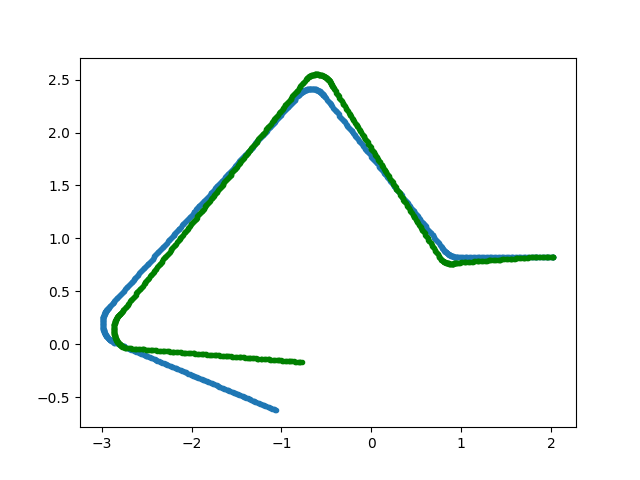
\includegraphics[width=0.22\textwidth]{figuras/M1C1NotWeighted.png}} \hspace{0.1cm}
\subfigure[Circuit 01 with filtering ($ c = 1.05 $).]{\label{fig:M1C1W}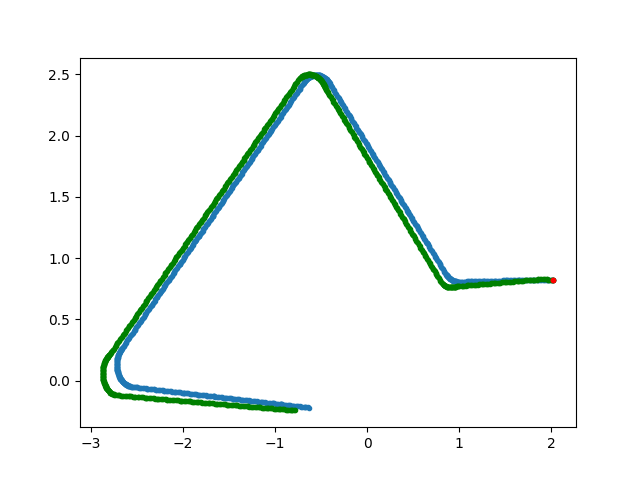
\includegraphics[width=0.22\textwidth]{figuras/M1C1Weighted.png}} \\
\subfigure[Circuit 02 without filtering.]{\label{fig:M1C2NW}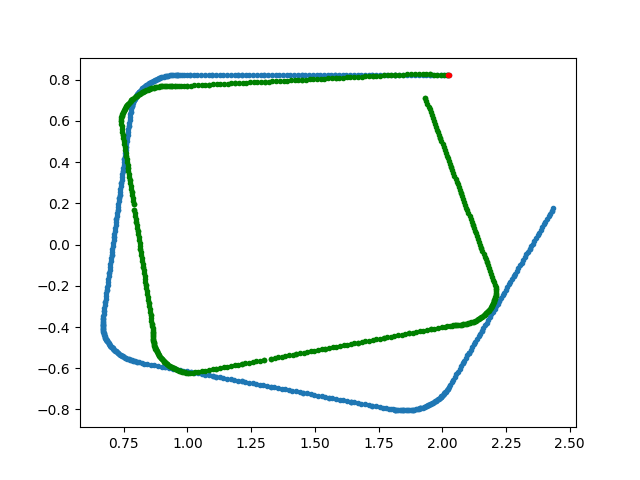
\includegraphics[width=0.22\textwidth]{figuras/M1C2NotWeighted.png}}
\subfigure[Circuit 02 with filtering ($ c = 1.05 $).]{\label{fig:M1C2W}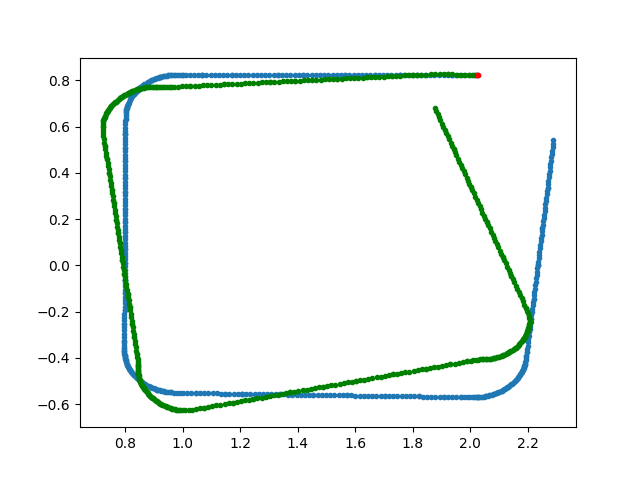
\includegraphics[width=0.22\textwidth]{figuras/M1C2Weighted.png}}
\caption{Result of Odometry using only encoders with and without angle filtering.}
\label{fig:encoders_odometry}
\end{center}
\end{figure}


\subsection{Odometry only with gyroscope}
In this setup, we applied almost all the calculations of the previous one with only one difference: $ \Delta \theta $ is
get directly from the gyroscope without using any information from the encoders. The encoders are still being used to get
the angle variation on the wheels but those results are only used to calculate $ \Delta x $ and $ \Delta y $. The idea
is to try to check the behaviour of the predicted trajectory using another sensor to help. In order to have a fair comparison,
we kept all the same trajectories from the previous approach. The results are shown in the figure \ref{fig:encoders_gyroscope}.

\begin{figure}[h]
\begin{center}
    % \centering     %%% not \center
\subfigure[Circuit 01 without filtering.]{\label{fig:M2C1NW}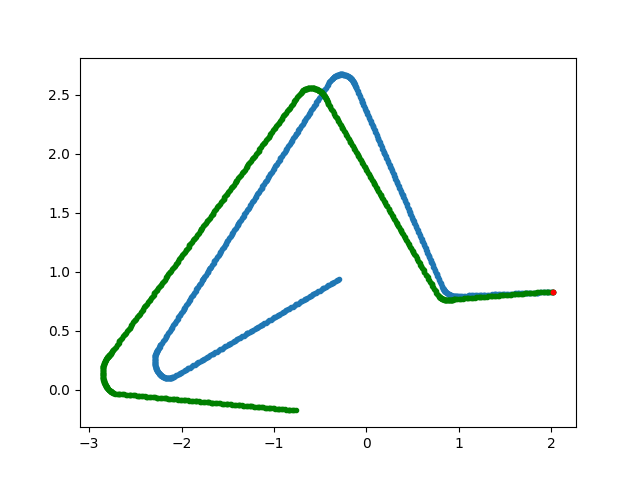
\includegraphics[width=0.22\textwidth]{figuras/M2C1NotWeighted.png}} \hspace{0.1cm}
\subfigure[Circuit 01 with filtering ($ c = 0.85 $).]{\label{fig:M2C1W}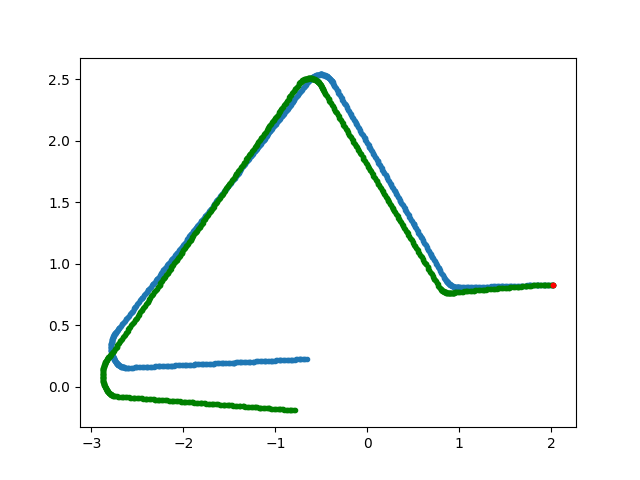
\includegraphics[width=0.22\textwidth]{figuras/M2C1Weighted.png}} \\
\subfigure[Circuit 02 without filtering.]{\label{fig:M2C2NW}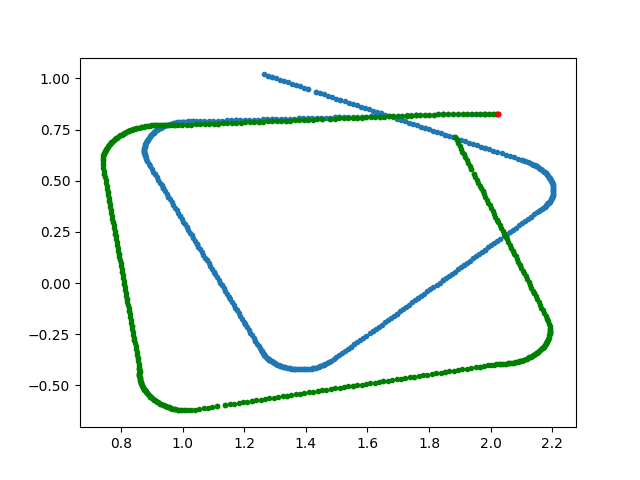
\includegraphics[width=0.22\textwidth]{figuras/M2C2NotWeighted.png}}
\subfigure[Circuit 02 with filtering ($ c = 0.85 $).]{\label{fig:M2C2W}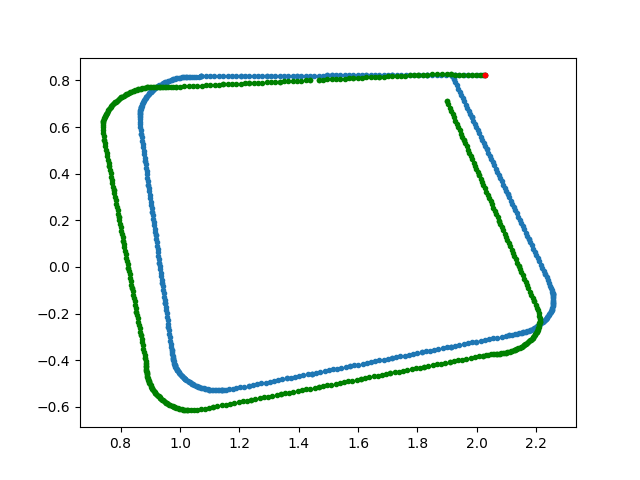
\includegraphics[width=0.22\textwidth]{figuras/M2C2Weighted.png}}
\caption{Result of Odometry using only gyroscope with and without angle filtering.}
\label{fig:encoders_gyroscope}
\end{center}
\end{figure}

\subsection{Odometry with encoders and gyroscope (Sensor Fusion)}
After applying the two previous strategies, we can see that each one still have errors more associated to the curves of the trajectory. More specificaaly, 
setup with only encoders tends to predict angles lower than the real ones performed
by the robot as long as the setup only with gyroscope tends to predict angles greater than the ones in ground truth.
This can be easier checked when we compare the figures \ref{fig:M1C2NW} and \ref{fig:M2C2NW}. Even after applying the 
filtering process in the angles, we got lower errors but the same conclusions remain for encoders and gyroscope 
strategies. Therefore we decied to put the both together in order to achieve a best result. Now the $ \Delta \theta $ is 
obtained through the following equations to fuse both result sensors:

\begin{equation}
  \Delta \theta_{fusion} = (\Delta \theta_{enco} + \Delta \theta_{gyros})/2
  \label{equation:fusion01}
\end{equation}

\begin{equation}
  \Delta \theta_{fusion} = (c_{enco}.\Delta \theta_{enco} + c_{gyro}. \Delta \theta_{gyro})/2
  \label{equation:fusion02}
\end{equation}

Where $ \Delta \theta_{enco} $ is the angle variation obtained using the encoders, $ \Delta \theta_{gyro} $
is the angle variation using gyroscope, $ c_{enco} $ and $ c_{gyro} $ are the factors that multiply each angle 
in the weighted sensor fusion. Since the filtering has been a good way to reduce error, as we will explain in the following subsection, we applied the
same idea weighting each of the angle variations and taking the mean as shown in equation \ref{equation:fusion02}. The
results of the fusion are in the Figure \ref{fig:encoders_fusion}. 

\begin{figure}[h]
\begin{center}
    % \centering     %%% not \center
\subfigure[Circuit 01 without filtering.]{\label{fig:M3C1NW}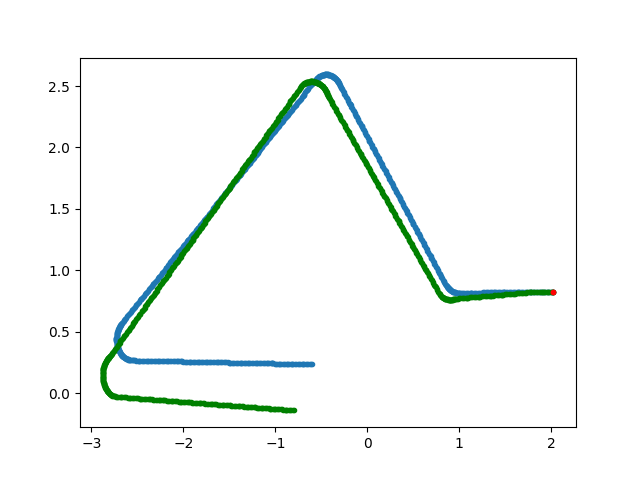
\includegraphics[width=0.22\textwidth]{figuras/M3C1NotWeighted.png}} \hspace{0.1cm}
\subfigure[Circuit 01 with filtering ($ c_{enco} = 1.05 $ and $ c_{gyro} = 0.90 $).]{\label{fig:M3C1W}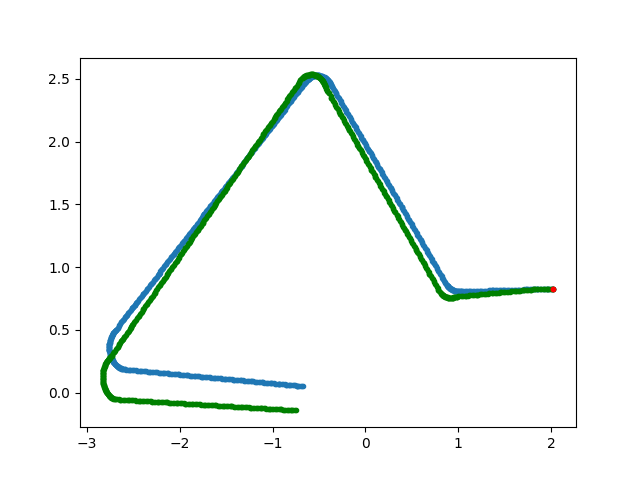
\includegraphics[width=0.22\textwidth]{figuras/M3C1Weighted.png}} \\
\subfigure[Circuit 02 without filtering.]{\label{fig:M3C2NW}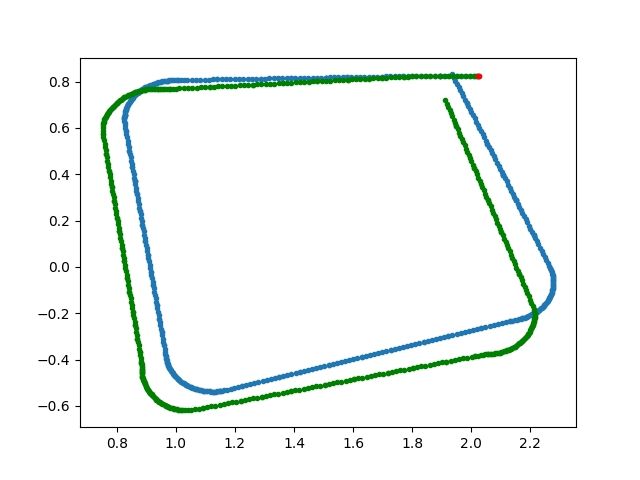
\includegraphics[width=0.22\textwidth]{figuras/M3C2NotWeighted.png}}
\subfigure[Circuit 02 with filtering ($ c_{enco} = 1.05 $ and $ c_{gyro} = 0.90 $).]{\label{fig:M3C2W}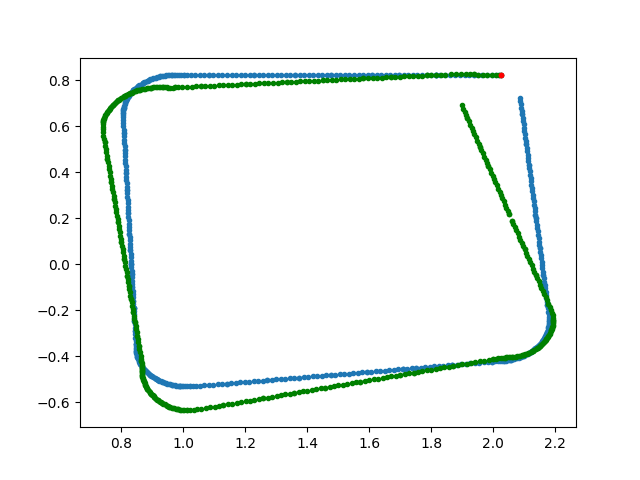
\includegraphics[width=0.22\textwidth]{figuras/M3C2Weighted.png}}
\caption{Result of Odometry using fusion of encoders and gyroscope.}
\label{fig:encoders_fusion}
\end{center}
\end{figure}

\subsection{Discussion of the results}
In the first setup based only on encoders, we can see that the error increases mainly after a curve that changes the 
trajectory in ninety or more degrees. This is because the way that the angle variations are calculated: the encoder of
a wheel takes the initial angle, wait for a little time, and takes again the final angle and then the code perfoms
the subtraction and get the $ \Delta \phi $ variation in each wheel. During a curve, maybe it does not have enogh time
to calculate, in each calling to the function, all the possible variations of the wheel that runs the further distance,
since we are making the curve setting a wheel to zero and the another one to a velocity greater than zero (we always used $ 2.0 $). So the wheel with higher velocity will run the greater distance and then the encoders cannot
take in the account all of the variations. It leads to mispredictions of trajectories that turns angles lower than the real ones as we can see mainly in figures \ref{fig:M1C1NW} and \ref{fig:M1C2NW}. With filtering, the error is smoothed, by increasing the value of the angle multypling it by a fcator higher than $ 1.0 $, but
we still have some great diferences mainly in the middle and in the end of trajectory since the error is propagated
to the future steps of the odometry. Even if the prediction in a specific point is good, the summation of previous
erros might overcome this right prediction. We can easier see this in figure \ref{fig:M1C2W} in the end of the 
trajectory. The first circuit with filtering is almost perfect due to the fact that we have a lower distance 
to be travelled which allow us to have a lower accumulated error and only two curves with angles higher than ninety
degrees (the second and last ones). Figure \ref{fig:M1C1W} illustrates this explanation. \par
In the second setup using only the gyrsocope, we have the opposite behaviour of the preious one: higher predicted
angles compared to the real ones. We can see this in Figures \ref{fig:M2C1NW} and \ref{fig:M2C2NW}. We think this
is related to the greater sensibility of the gyroscope in which it reports lower variation angles than the encoders
but in a higher frequency and then we have erros acumullated faster in the curves. Therefore, in contrast to previous
setup, we multiply the angles by a factor lower than $ 1.0 $ in order to get lower angles to be added to the odometry. 
Figures \ref{fig:M2C1W} and \ref{fig:M2C2W} can illustrate that the results are improved a lot but due to the sensibility, noise, and some assynchronous behavious we still have errors. \par
Compared to the first setup, the second one is a little worse, however, they are complementars, that is, the former
predict angles lower than the real ones and the last predicts angles higher than the groud truth. So the combination
of the them seems promising in a way that we can fuse them in a single result and get a better prediction. The results
without any filtering and combining them using equation \ref{equation:fusion01} is showed in figures \ref{fig:M3C1NW} and \ref{fig:M3C2NW}. As we expected, the resulting odometries for each circuit is closert o the ground truth when we 
compared to the other non-filtered circuits. We have little improvement when comparing \ref{fig:M1C1NW} and \ref{fig:M2C1NW} to \ref{fig:M3C1NW} due to the lower distance of the circuit $ 01 $ compared to the cirucit $ 02 $. In this
last one we see a higher improvement with fusion not only in the endpoint but also along all the trajectory which the
robot remained cosed to the ground truth. To be fair, we also applied the filtering strategy in the fusion using one factor to each angle (Equation \ref{equation:fusion02}). The factors are shown in the captions of the Figures \ref{fig:M3C1W} and \ref{fig:M3C2W}. We see that for the first circuit we had a worse result, so encoders are better to be
used in shorter distances with smoother angles. But ofr the circuit $ 02 $ which is longer only with ninety-degree curves, we see a better behaviour along the trajectory mainly in the curves which are better predicted and well shaped,
even with a further endpoint compared to the gyroscope alone (Figure \ref{fig:M2C2W}). \par
Now that we exposed our conclusions to shorter distances, we will present the performance considering the trajectory
used in Points Extraction of the scene, since it has angles in different degrees and covers almost all rooms and longer
distances.

\section{Putting it togheter: Points Extraction with Odometry}
Now that we have exposed all of the explanations and results of Points Extraction and Odometry, we will evaluate the
odometry setups in a higher distance, with angles in different degrees, longer distances and covering almost all the
enviorment. This will put in a higher test, since the erros tends to be higher as the distance and angles degrees
increase. Since the filtering strategy was the better for the three setups, we only shows the results to them. Figure
\ref{fig:encoders_fusion_extraction_points} shows the results.  

\begin{figure}[h]
\begin{center}
    % \centering     %%% not \center
\subfigure[Odometry based only on encoders.]{\label{fig:M1C3W}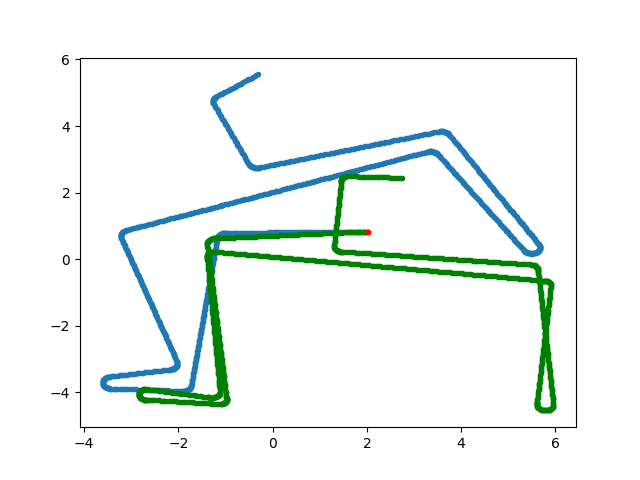
\includegraphics[width=0.22\textwidth]{figuras/M1C3Weighted.png}} \hspace{0.1cm}
\subfigure[Odometry based onlt on gyrosocope.]{\label{fig:M2C3W}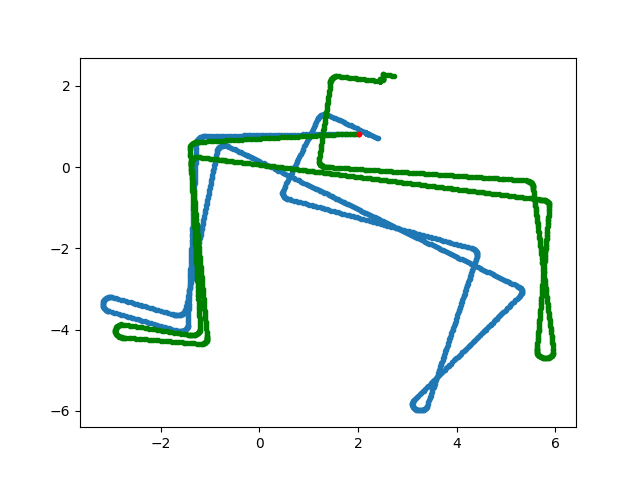
\includegraphics[width=0.22\textwidth]{figuras/M2C3Weighted.png}} \\
\subfigure[Odometry with fusion.]{\label{fig:M3C3W}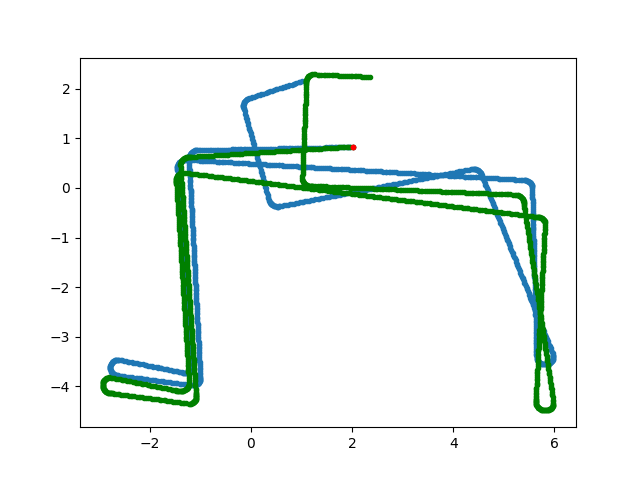
\includegraphics[width=0.22\textwidth]{figuras/M3C3Weighted.png}}
\caption{Odometry result for each setup with filtering.}
\label{fig:encoders_fusion_extraction_points}
\end{center}
\end{figure}

As previously concluded, even with filtering, setup with encoders tends to predict angles lower than the ground truth,
and then in each curve (mainly in sharp curves) the error increases and eu to the longer distances, we have more 
accumulation of erros, and then teh final result is very different from the ground truth (Figure \ref{fig:M1C3W}). This 
enforces our previoius conclusion: encoders are better in shorter distances and lower angles. Following the same way of 
first setup, the second one based only on gyroscope still leads to high erros because of the same reason that we have 
already discussed: predicts higher angles possibly due to ythe sensibility (Figure \ref{fig:M2C3W}). However, as we were 
expecting, the fusion with filtering from both sensors gives us the best odometry as illustrated in Figure \ref{fig:M3C3W}. Along almost all the trajectory the robot keeps closer to the ground truth accumulating lower erros with little 
deviation. During the turns the robot keeps closer to the expected trajectory without big discrenpancies as we saw two 
the previous ones. Therefore, the sensor fusion gave us the best performance and tends to get good results in further 
trajectories.


\section{Feature Extraction}

As the robot acquires information from the environment, the data must be processed in order to be useful in more complex actions such as decision making, mapping, navigation. In the case of autonomous robots, the distance points obtained from a variety of sensors can be used to deduce obstacles and landmarks in the environment, such as walls, doors, supports of objects, and so on. The recognition of those structures is fundamental to solve its main actions, like identifying victims in a desaster scenario, delivering resources in an unknown environment, robust mapping withoud human interference.
\par In our case, the 2D LIDAR sensor was used to obtain obstacle points related to the robot frame, and then converted to the global frame, as mentioned in the previous subsection. As the number of obtained points is huge (order of $10^{6}$ samples for full exploration of our test scene), an algorithm for extracting line features from those points was implemented, based on the idea of Random Sample Consensus (RANSAC\cite{fischler1981random}). As a result, it is desired to obtain a map of line features representing obstacles in the enviroment, which could be later used in an Occupation Grid algorithm for mapping, and as landmarks in a A* algorithm for navigation, for example. The main implementation decisions are listed next. 

\subsection{Feature Extraction Trigger}
To execute the Feature Extraction step for implementation, it was decided to do it offline, which is, after the exploration step is concluded. Even though this is a naive solution and possibly would not be recomended for real operations, it is a good choice for prototyping and validation of the algorithm. So, when discussing the execution pipeline, after the exploration and data acquirement step, the output points with respect to the global reference frame is saved and used as input to the Feature extraction algorithm, named \textbf{feature\_extraction.py}. Then, it starts its execution.

\subsection{Line Calculation with RANSAC}

In order to find lines, the obstacle points are order with respect to their x and y coordinates,and then the RANSAC algorithm starts operating. As we are dealing with lines in the cartesian plane, the method struggles when trying to resolve vertical lines. To fix this issue, the algorithm executes two times, one for the regular $xy$ plane, and another for the inverted $yx$ plane, to be able to find the vertical ones. The names of the RANSAC execution functions inside the code are \textit{ransac\_regular\_plane} and \textit{ransac\_inverted\_plane}. The inputs for the functions are the obstacle points. As their functioning is almost the same (with the difference of with type of lines they calculate), a general explanation of the case for the regular plane is given.
\par For a predefined number of execution times, two points from the obstacle points list are taken randomly, and then a line crossing both points are considered. For every point in the set, if the point is close enough to the line (considering a threshold), the point is considered to belong to that respective line, and then saved in other structure. If the number of points (hit points) is high enough (considering a specific metric), we probably have a line. Analyzing those hit points, as they fit the calculated line, it is known that they are colinear enough, but not necessarily close enough to belong to the same structure (like a door, wall). Therefore, those points are passed through and the distance between neighbors is checked. If two consecutive neighbors are close enough (with respect to a metric), they probably belong to the same line. If not, we probably found a discontinuity. If the discontinuity is found, the number of consecutive points found until this step is counted. If they are greater than a metric, a line has been found. If not, those consecutive points are discarded, as they are probably outliers. If any lines have been found, they are stored by saving the $x,y$ of the first point that fits the line and the $x, y$ of the last point that fits that same line. So the algorithm returns a list of lines, in which every element contains a list with the following chracteristics: $
\begin{bmatrix}x_{firstPoint} & y_{firstPoint} & x_{lastPoint} & y_{lastPoint}\end{bmatrix}
$. Pseudocode is shown in algorithm \ref{code:ransac}

\begin{algorithm}
    \caption{RANSAC}\label{code:ransac}
    \begin{algorithmic}[1]
        \Procedure{RANSAC(points)}{}
        \While{$loop\_idx < MAX\_ITER$}
        \State $guess[2] \gets random(points)$
        \State $line\_incl \gets (point[0].y - point[1].y)/(point[0].x - point[1].y)$
        \State $cross\_y \gets point[1].y + point[1].x*((point[0].y - point[1].y)/(point[1].x - point[0].x))$

        \For{$point\ in\ points$}
            \State $d.append(CALCULATE\_DISTANCE$
            $(point,\ line\_incl,\ cross\_y))$
        \EndFor
        \State $d \gets NORMALIZE\_DISTANCE(d)$

        \For{$distance\ in\ d$}
            \If{$distance < DIST\_THRESHOLD$}
                \State $hit\_rate \gets hit\_rate + 1$
                \State $hit\_idx.append(distance)$
            \EndIf
        \EndFor

        \If{$hit\_rate > MIN\_HITS$}
            \For{$idx\ in\ hit\_idx$}
                \State $d\_between\_points \gets DISTANCE(point[idx],\ point[idx - 1])$
                \If {$d\_between\_points > MAX\_D$}
                    \If {$n\_points > MIN\_CONS\_P$}
                        \State $lines.append(LINE(start,\ points[idx]))$
                    \EndIf
                \Else
                    \State $n\_points \gets n\_points + 1$
                \EndIf
                \State $start \gets point[idx]$
            \EndFor
        \EndIf

        \State $loop\_idx \gets loop\_idx + 1$
        \EndWhile
        \EndProcedure
    \end{algorithmic}
\end{algorithm}
The threshold to analyze if points are close to the calculated line is done by taking the distance from all points in the set to the line, and then normalizing them. If the normalized distance to the point is below $10\%$, the point is considered belonging to the line. The number of minimum points necessary to form a line was chosen empirically, with the value of $10000$. The number of minimum consecutive points to form a line was also defined empirically, with the value of $1000$.

\subsection{Line merging and Printing}
After calculating the lines, one last attempt is done of trying to merge lines that are colinear and close enough. The obtained lines are ordered, and every line is checked with its right neighbor, to analyze if they are colinear and close enough. The metrics for comparison where obtained empirically. If they do, they are merged into a single one. If they do not, the line is painted on canvas for user output, but its parameters could be easily saved for usage in other modules. The process is done for lines in regular and inverted plane. 

\subsection{Experiments and Results}

For features extracted from our test scene, the group uses the points selected from the exploration step, as mentioned before. For printing the lines, in other to make it easier for the reader to analyze the output, a canvas 1024x1024 pixels is created, and then the lines are written in blue color. To make it comparable with the points, figure \ref{fig:canvas-points} shows the canvas painted with the original points obtained by the sensors, in which every pixel represents one or more incidences. Figures \ref{fig:canvas-features} shows the execution of the algorithm for 10, 50 and 100 RANSAC iterations. 

\begin{figure}[H]
    \centering
    \includegraphics[scale=0.5,width=0.5\hsize]{figures/points.png}
    \caption{Canvas with extracted points painted on it}
    \label{fig:canvas-points}
\end{figure}


\begin{figure}[H]
    \centering
    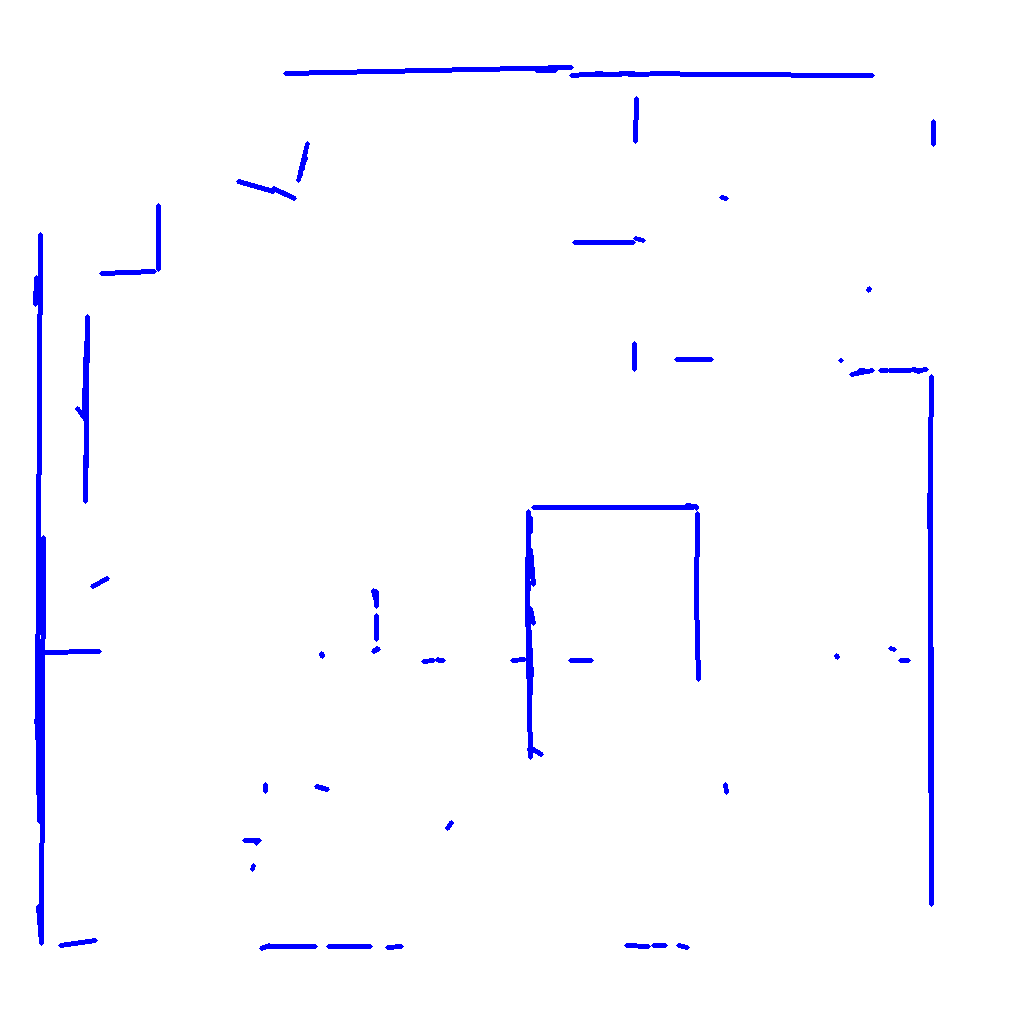
\includegraphics[scale=0.5,width=0.5\hsize]{figures/all_features-10-iter.png}
    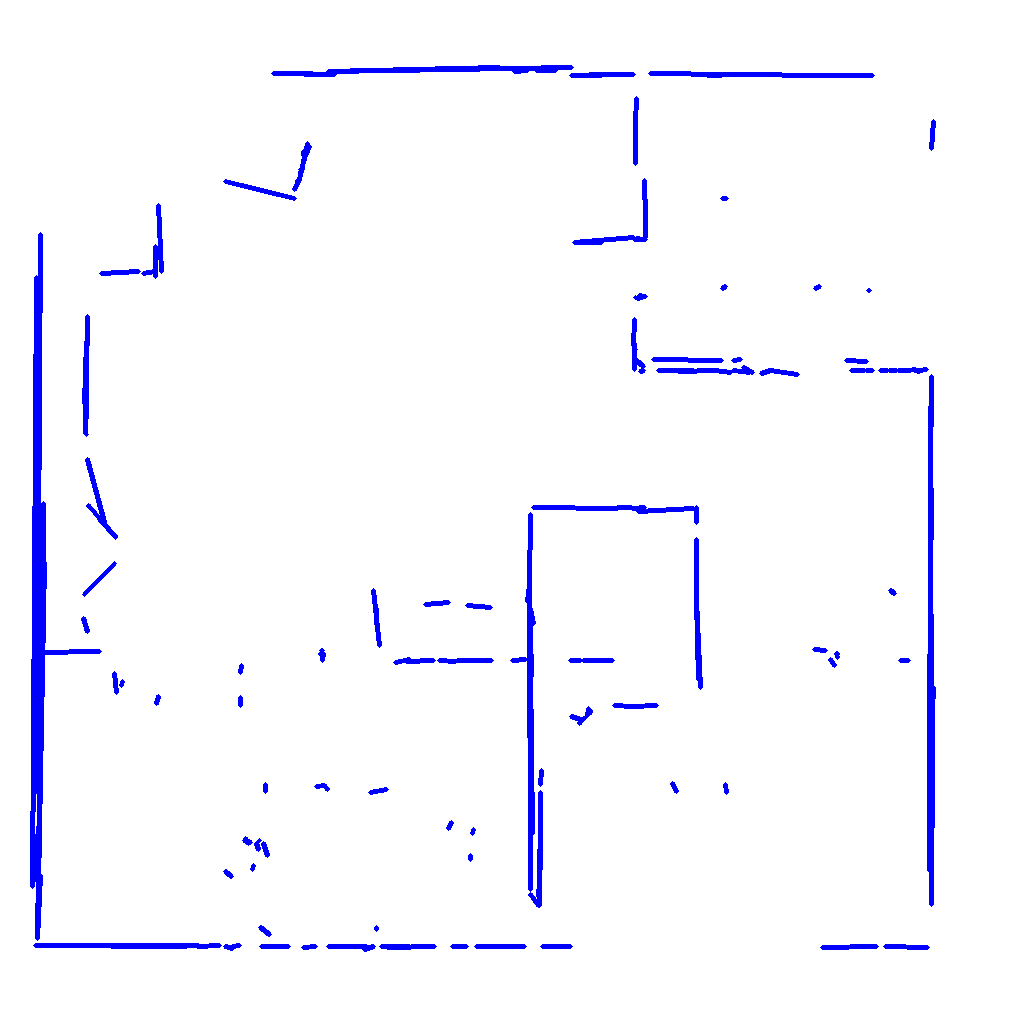
\includegraphics[scale=0.5,width=0.5\hsize]{figures/all_features-50-iter.png}
    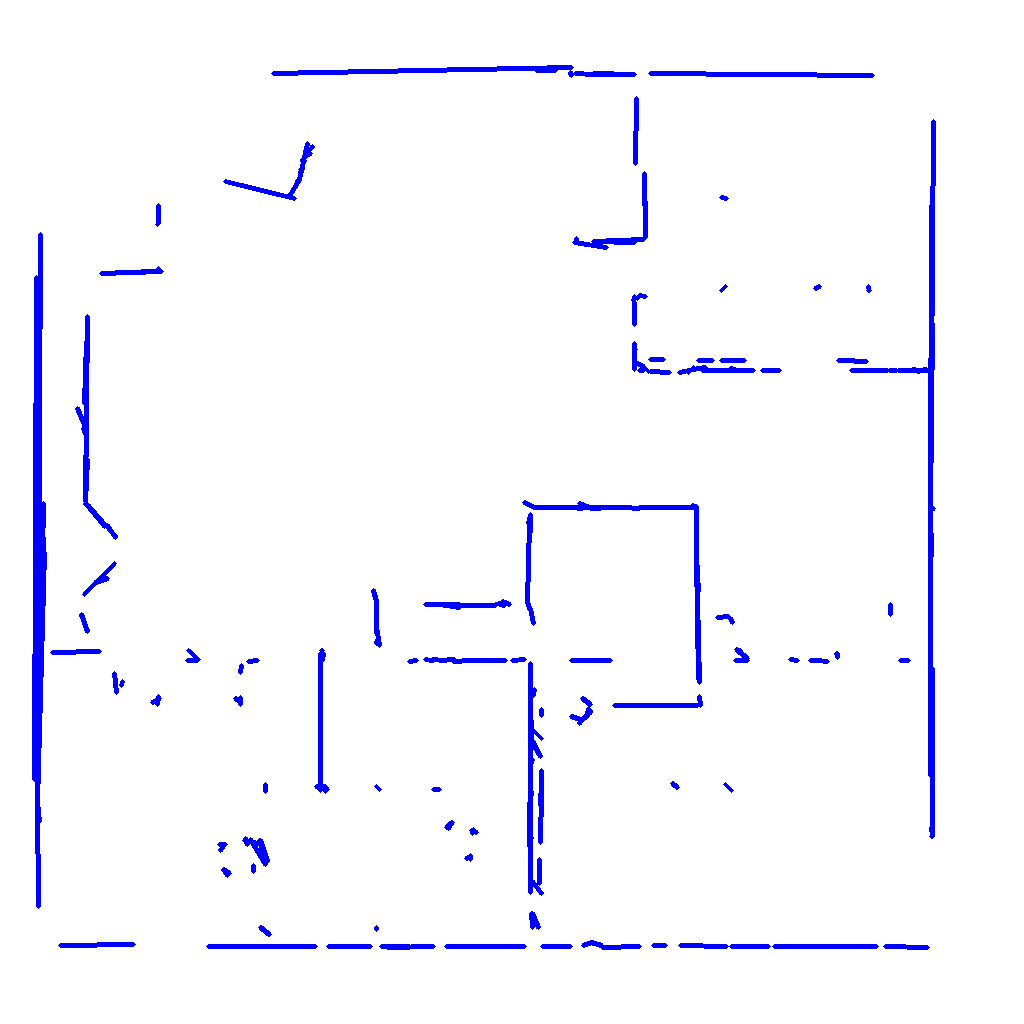
\includegraphics[scale=0.5,width=0.5\hsize]{figures/all_features-100-iter.png}
    \caption{Canvas with extracted features. a) 10 RANSAC iterations. b) 50 RANSAC iterations. c) 100 RANSAC iterations}
    \label{fig:canvas-features}
\end{figure}

From the output images, it is possible to conclude that the RANSAC method can build features from the points with good consistency. The more iterations, the greater is the number of features built. As the method is sthocastic, the features change from execution to the other, so one interesting strategy is to guarantee a minimum number of execution times to extract all main features.
\par The line merging approach, although it is able to perform its objective sometimes, still needs to be improved, as it produces false positives in some cases (\textit{e.g.: }false vertical line in bottom left room of canvas, connecting two support feet of table, for 100 iterations case). 
\par A great number of features was not fully produced, as we can see some incomplete walls in Figure \ref{fig:canvas-features}. The possible reasons for these cases are: lack of treatment for noisy data acquirement, poor strategy at choosing guess candidates (as we have $10^{6}$ points magnitude), bad parameter tuning (as the majority of the comparison parameters where set empirically). The "brute force" strategy, which consists of doing a greater number of RANSAC iterations (approx. 500 times), showed to be innefective as a trial to produce more features, which shows that fixing some of the problems could improve our results.

\section{Conclusion}
The implementation of odometry and feature extraction modules to autonomous mobile robotics allowed us to understand some of the challenges in the area. 
\par The module built to extract points from the action environment showed to be adequate, given the fact that the robot position is known. The odometry module also showed good results when sensor fusion was performed. It was able to see in practice the problems related to odometry solutions when relying on few sensors. The feature extraction module returned good results, and presents great opportunity for improvement in the line selection strategies.
\par Overall, the project was a great opportunity to get used to the tools explored in the area, and provided base material for future improvements, considering that more complex actions will be implemented for the robot during the semester.  

 +-------------+

\bibliographystyle{IEEEtran}

\bibliography{Relatorio}


%******************************************************************************

%\vspace{20ex}

%\section*{\Large \textbf{Submissão}}

%Seu trabalho deve ser submetido via moodle em conjunto com o có digo fonte.

%\vspace{3ex}


\end{document}
